\documentclass[12pt,a4paper]{report}

% =========================================================================
% GOI THU VIEN & CAU HINH CO BAN
% =========================================================================
\usepackage{fontspec}
\setmainfont{Times New Roman}

\usepackage[top=2.5cm,bottom=2.5cm,left=3.0cm,right=2.0cm]{geometry}
\usepackage{amsmath,amsfonts,amssymb}
\usepackage{graphicx}
\usepackage{booktabs}
\usepackage{tabularx}
\usepackage{multirow}
\usepackage{array}
\usepackage{float}
\usepackage{xcolor}
\usepackage{tikz}
\usetikzlibrary{calc,positioning,shapes.geometric,arrows.meta}
\usepackage{hyperref}
\usepackage{fancyhdr}
\usepackage{titlesec}
\usepackage{caption}
\usepackage{subcaption}
\usepackage{enumitem}
\usepackage{listings}
\usepackage{tcolorbox}

\graphicspath{{images/generated/}{images/}}

% Cau hinh Hyperref
\hypersetup{
    colorlinks=true,
    linkcolor=blue!80!black,
    citecolor=green!60!black,
    urlcolor=blue!70!black,
    pdftitle={Bao Cao Ky Thuat Assignment 04 - Convolutional Neural Networks},
    pdfauthor={khoipv.447}
}

% Cau hinh Code Listing cho Python / NumPy
\definecolor{codegreen}{rgb}{0,0.6,0}
\definecolor{codegray}{rgb}{0.5,0.5,0.5}
\definecolor{codepurple}{rgb}{0.58,0,0.82}
\definecolor{backcolour}{rgb}{0.96,0.97,0.98}

\lstdefinestyle{mystyle}{
    backgroundcolor=\color{backcolour},
    commentstyle=\color{codegreen},
    keywordstyle=\color{blue!80!black}\bfseries,
    numberstyle=\tiny\color{codegray},
    stringstyle=\color{codepurple},
    basicstyle=\ttfamily\footnotesize,
    breakatwhitespace=false,
    breaklines=true,
    captionpos=b,
    keepspaces=true,
    numbers=left,
    numbersep=5pt,
    showspaces=false,
    showstringspaces=false,
    showtabs=false,
    tabsize=2,
    frame=single,
    rulecolor=\color{black!20}
}
\lstset{style=mystyle}

% Dinh dang tieu de chuong, muc
\titleformat{\chapter}[display]
  {\normalfont\bfseries\color{blue!80!black}}
  {\filleft\Large\bfseries\chaptertitlename\ \thechapter}
  {1ex}
  {\titlerule\vspace{1ex}\filright\LARGE}
  [\vspace{1ex}\titlerule]

\titleformat{\section}
  {\normalfont\Large\bfseries\color{blue!70!black}}
  {\thesection}{1em}{}

\titleformat{\subsection}
  {\normalfont\large\bfseries\color{black!85}}
  {\thesubsection}{1em}{}

% Header & Footer
\pagestyle{fancy}
\fancyhf{}
\fancyhead[R]{\small\itshape Assignment 04: Convolutional Neural Networks}
\fancyfoot[C]{\thepage}
\renewcommand{\headrulewidth}{0.4pt}
\renewcommand{\footrulewidth}{0.4pt}
\setlength{\headheight}{14pt}

\newcommand{\modelpath}[1]{\texttt{#1}}
\newcommand{\best}[1]{\textbf{#1}}
\newcommand{\notebookname}[1]{\textit{#1}}

% =========================================================================
% BAT DAU TAI LIEU
% =========================================================================
\begin{document}

% -------------------------------------------------------------------------
% TRANG BIA
% -------------------------------------------------------------------------
\hypersetup{pageanchor=false}
\begin{titlepage}
\thispagestyle{empty}
\begin{tikzpicture}[remember picture,overlay]
    \draw[line width=1.1pt]
      ($(current page.north west)+(1.45cm,-1.35cm)$)
      rectangle
      ($(current page.south east)+(-1.45cm,1.35cm)$);
    \draw[line width=0.35pt]
      ($(current page.north west)+(1.60cm,-1.50cm)$)
      rectangle
      ($(current page.south east)+(-1.60cm,1.50cm)$);
\end{tikzpicture}

\begin{center}
    \textbf{\fontsize{16}{20}\selectfont
    HỌC VIỆN CÔNG NGHỆ BƯU CHÍNH VIỄN THÔNG}\\[0.15cm]
    \textbf{\fontsize{15}{19}\selectfont KHOA CÔNG NGHỆ THÔNG TIN 1}\\[0.25cm]
    \rule{4cm}{0.4pt}

    \vspace{0.75cm}
    % Logo chu duoc ve truc tiep de file bao cao tu chu, khong phu thuoc asset bia.
    
\begin{tikzpicture}
        \node[
            text=red!80!black,
            font=\bfseries\fontsize{30}{34}\selectfont,
            inner sep=1pt
        ] (ptit) {PTIT};
        \node[
            star,
            star points=5,
            star point ratio=2.2,
            fill=yellow!85!orange,
            draw=yellow!60!black,
            minimum size=0.72cm,
            inner sep=0pt
        ] at ($(ptit.north)+(0.18cm,-0.06cm)$) {};
        \draw[red!80!black,line width=1.1pt]
            ($(ptit.south west)+(-0.10cm,-0.18cm)$) --
            ($(ptit.south east)+(0.10cm,-0.18cm)$);
        \draw[red!80!black,line width=0.45pt]
            ($(ptit.south west)+(-0.10cm,-0.25cm)$) --
            ($(ptit.south east)+(0.10cm,-0.25cm)$);
    \end{tikzpicture}

    \vspace{0.55cm}
    \textbf{\fontsize{17}{21}\selectfont BÁO CÁO MÔN HỌC}\\[0.25cm]
    \textbf{\fontsize{17}{21}\selectfont PHÁT TRIỂN CÁC HỆ THỐNG THÔNG MINH}\\[0.40cm]
    \textbf{\fontsize{17}{21}\selectfont ASSIGNMENT 04}

    \vspace{1.15cm}
    \begin{tabular}{>{\bfseries}p{3.8cm}p{6.2cm}}
        Họ tên: & Phan Văn Khôi \\
        Mã sinh viên: & B23DCCN447 \\
        Lớp: & D23CTPM01-B \\
        Giảng viên: & PGS. TS. Trần Đình Quế \\
    \end{tabular}

    \vfill
    \textbf{\fontsize{14}{18}\selectfont Hà Nội -- 2026}
\end{center}
\end{titlepage}
\hypersetup{pageanchor=true}

% -------------------------------------------------------------------------
% MUC LUC & DANH MUC HINH ANH / BANG BIEU
% -------------------------------------------------------------------------
\pagenumbering{roman}
\tableofcontents
\newpage
\listoffigures
\newpage
\listoftables
\newpage
\pagenumbering{arabic}

% -------------------------------------------------------------------------
% THONG TIN PROJECT
% -------------------------------------------------------------------------
\chapter*{Thông Tin Project}
\addcontentsline{toc}{chapter}{Thông Tin Project}

\noindent\textbf{GitHub project:} \url{https://github.com/KhoiF/PTHTTM}

\vspace{0.4cm}
\noindent
Repository lưu mã nguồn notebook, dữ liệu cục bộ, hình ảnh sinh từ thực nghiệm và báo cáo \LaTeX{} của Assignment 04.
Hai notebook được sử dụng làm nguồn duy nhất cho các số liệu trong báo cáo là:
\begin{itemize}
    \item \modelpath{src/Assignment 04/mnist/notebook/mnist\_cnn\_benchmark.ipynb};
    \item \modelpath{src/Assignment 04/cifar10/notebook/cifar10\_cnn\_benchmark.ipynb}.
\end{itemize}

\noindent
Mỗi notebook huấn luyện ba cách cài đặt: CNN thuần NumPy, TensorFlow/Keras và PyTorch.
Các hình trong báo cáo được lấy từ output đã sinh của chính hai notebook và đặt tại
thư mục \modelpath{images/generated} của Assignment 04.
\newpage

% =========================================================================
% CHUONG 1
% =========================================================================
\chapter{Cơ Sở Lý Thuyết Về Mạng Nơ-ron Tích Chập}

\section{Bài toán phân loại ảnh}
Một ảnh số có thể biểu diễn bằng tensor
$\mathbf{X}\in\mathbb{R}^{H\times W\times C}$,
trong đó $H$, $W$ và $C$ lần lượt là chiều cao, chiều rộng và số kênh màu.
Bài toán phân loại ảnh học một hàm tham số $f_{\theta}$ để ánh xạ ảnh sang phân phối xác suất trên $K$ lớp:
\begin{equation}
    \mathbf{X}
    \xrightarrow{f_{\theta}}
    \mathbf{z}\in\mathbb{R}^{K}
    \xrightarrow{\text{softmax}}
    \hat{\mathbf{y}}.
\end{equation}

Nếu dùng mạng fully connected ngay trên toàn bộ pixel, quan hệ lân cận bị phá vỡ khi ảnh được làm phẳng.
Số tham số cũng tăng nhanh theo độ phân giải.
Convolutional Neural Network (CNN) giải quyết hai hạn chế này bằng \textit{kết nối cục bộ} và \textit{chia sẻ trọng số}.
Cùng một kernel được quét trên nhiều vị trí nên có thể phát hiện một mẫu hình bất kể mẫu đó xuất hiện ở đâu trong ảnh.

\subsection{MNIST và CIFAR-10 như hai mức độ khó}
MNIST gồm ảnh xám $28\times28\times1$ của mười chữ số viết tay.
Nền tối, vật thể đơn và hình dạng chữ số rõ khiến đây là bộ dữ liệu phù hợp để kiểm tra tính đúng đắn của một CNN tự cài đặt.

CIFAR-10 gồm ảnh màu $32\times32\times3$ thuộc mười nhóm vật thể tự nhiên.
Ảnh có nền phức tạp, góc nhìn và hình dạng đa dạng, trong khi độ phân giải thấp.
Vì vậy mô hình phải học cả cạnh, texture, màu sắc và cấu trúc cấp cao hơn.
Sự chênh lệch độ khó giữa hai bộ dữ liệu là cơ sở tốt để đánh giá giới hạn của CNN nông và lợi ích của residual learning.

\section{Phép tích chập và feature map}
Với kernel kích thước $K_h\times K_w$, stride $S$ và padding $P$, phần tử tại vị trí $(i,j)$ của feature map thứ $k$ được tính bởi:
\begin{equation}
Y_{i,j,k}=b_k+
\sum_{u=0}^{K_h-1}
\sum_{v=0}^{K_w-1}
\sum_{c=0}^{C-1}
X_{iS+u-P,\,jS+v-P,\,c}W_{u,v,c,k}.
\end{equation}

Nếu đầu vào có kích thước $H\times W$, kích thước không gian đầu ra là:
\begin{align}
H_{out} &= \left\lfloor\frac{H+2P-K_h}{S}\right\rfloor+1,\\
W_{out} &= \left\lfloor\frac{W+2P-K_w}{S}\right\rfloor+1.
\end{align}
Padding \texttt{same} với kernel $3\times3$ và stride 1 giữ nguyên chiều cao, chiều rộng.
Trong hai notebook, các lớp convolution dùng kernel $3\times3$ để cân bằng khả năng học đặc trưng và chi phí tính toán.

\subsection{ReLU, pooling và receptive field}
Sau convolution, ReLU tạo tính phi tuyến:
\begin{equation}
    \operatorname{ReLU}(z)=\max(0,z).
\end{equation}
Max pooling $2\times2$ chọn kích hoạt lớn nhất trong từng vùng và giảm một nửa kích thước không gian.
Khi nhiều convolution được xếp chồng, receptive field tăng dần; neuron ở tầng sâu có thể tổng hợp thông tin từ vùng lớn hơn của ảnh gốc.

Với CNN NumPy trong notebook, chuỗi xử lý có dạng:
\begin{equation}
\text{Conv} \to \text{ReLU} \to \text{Pool}
\to \text{Conv} \to \text{ReLU} \to \text{Pool}
\to \text{Dense} \to \text{ReLU} \to \text{Dense}.
\end{equation}
Kiến trúc này đủ ngắn để hiện thực toàn bộ forward/backward nhưng vẫn có hai cấp feature map.

\section{Softmax và Cross-Entropy}
Với vector logits $\mathbf{z}$, softmax cho xác suất lớp $k$:
\begin{equation}
    \hat{y}_k=\frac{\exp(z_k)}{\sum_{j=1}^{K}\exp(z_j)}.
\end{equation}
Trong hiện thực số, notebook trừ $\max_j z_j$ trước khi lấy hàm mũ để tránh overflow.
Với nhãn one-hot $\mathbf{y}$, Cross-Entropy trên một batch $m$ mẫu là:
\begin{equation}
    \mathcal{L}_{CE}=-\frac{1}{m}\sum_{i=1}^{m}
    \sum_{k=1}^{K}y_{ik}\log(\hat{y}_{ik}+\epsilon).
\end{equation}
Đạo hàm kết hợp softmax và Cross-Entropy theo logits có dạng gọn
$\partial\mathcal{L}/\partial\mathbf{z}=\hat{\mathbf{y}}-\mathbf{y}$,
tạo điểm bắt đầu cho backpropagation qua dense, pooling và convolution.

\section{Backpropagation qua CNN}
Trong lớp convolution, gradient trọng số được cộng dồn từ mọi vị trí mà kernel đã được dùng.
Đây là hệ quả trực tiếp của parameter sharing.
Gradient theo đầu vào được phân phối ngược về các vùng ảnh tương ứng với từng cửa sổ convolution.

Với max pooling, chỉ vị trí đạt cực đại trong forward pass nhận gradient ở backward pass.
Notebook NumPy lưu mask cực đại để thực hiện phép phân phối này.
Các lớp dense dùng quy tắc đạo hàm ma trận quen thuộc:
\begin{align}
    \frac{\partial\mathcal{L}}{\partial\mathbf{W}}
    &=\mathbf{A}^{\top}\frac{\partial\mathcal{L}}{\partial\mathbf{Z}},\\
    \frac{\partial\mathcal{L}}{\partial\mathbf{b}}
    &=\sum_i\frac{\partial\mathcal{L}}{\partial\mathbf{Z}_i},\\
    \frac{\partial\mathcal{L}}{\partial\mathbf{A}}
    &=\frac{\partial\mathcal{L}}{\partial\mathbf{Z}}\mathbf{W}^{\top}.
\end{align}

\section{Các kỹ thuật cải thiện CNN}
\subsection{Batch Normalization và Dropout}
Batch Normalization chuẩn hóa activation theo mini-batch rồi học lại hệ số scale và shift.
Kỹ thuật này giúp quá trình tối ưu ổn định hơn và cho phép dùng learning rate lớn hơn.
Dropout ngẫu nhiên đặt một phần activation về 0 trong huấn luyện, qua đó giảm sự phụ thuộc quá mức giữa các neuron.
Mô hình framework cho MNIST dùng cả Batch Normalization và Dropout.

\subsection{Data augmentation}
Augmentation tạo biến thể hợp lệ của ảnh train mà không thay đổi nhãn.
MNIST dùng dịch chuyển ngẫu nhiên tối đa 2 pixel.
CIFAR-10 dùng reflect padding 4 pixel, random crop và horizontal flip xác suất 0.5.
Validation và test không augmentation, nhờ đó metric phản ánh khả năng tổng quát hóa trên dữ liệu gốc.

\subsection{Residual connection}
Một residual block học hàm $F(\mathbf{x})$ rồi cộng trực tiếp đầu vào:
\begin{equation}
    \mathbf{y}=F(\mathbf{x};\theta)+\mathbf{x}.
\end{equation}
Nếu kích thước hoặc số channel thay đổi, nhánh tắt dùng convolution $1\times1$ và stride tương ứng.
Đường truyền đồng nhất giúp gradient đi qua mạng sâu thuận lợi hơn.
Hai notebook dùng ResNet-20 cho CIFAR-10 với ba stage $16\to32\to64$, mỗi stage gồm ba residual block.

\subsection{Regularization và lịch learning rate}
L2 regularization bổ sung $\lambda\mathbf{W}$ vào gradient trọng số.
CNN NumPy còn clip từng phần tử gradient trong khoảng $[-5,5]$ và dùng Adam.
Learning rate của NumPy giảm theo cosine từ $10^{-3}$ xuống $5\times10^{-5}$.

MNIST framework dùng AdamW, learning rate ban đầu $10^{-3}$ và giảm khi validation metric ngừng cải thiện.
CIFAR-10 framework dùng SGD momentum 0.9, Nesterov, warm-up 5 epoch, cosine decay và label smoothing 0.1.
Các thành phần này đặc biệt quan trọng khi huấn luyện residual network trong 50 epoch.

\section{Các kiến trúc phát triển từ CNN}
\begin{table}[H]
\centering
\caption{Một số hướng phát triển tiêu biểu từ CNN cơ bản}
\label{tab:cnn_evolution}
\resizebox{\textwidth}{!}{%
\begin{tabular}{lll}
\toprule
\textbf{Kiến trúc} & \textbf{Cải tiến chính} & \textbf{Ý nghĩa} \\
\midrule
LeNet-5 & Conv, pooling và fully connected theo chuỗi & Nền tảng cho nhận dạng chữ số \\
AlexNet & ReLU, dropout, augmentation, GPU & Mở rộng CNN sâu lên ImageNet \\
VGG & Xếp chồng convolution $3\times3$ & Thiết kế đồng nhất nhưng nhiều tham số \\
Inception & Nhiều nhánh kernel và convolution $1\times1$ & Học đặc trưng đa tỉ lệ \\
ResNet & Skip/residual connection & Hỗ trợ mạng sâu, cải thiện luồng gradient \\
DenseNet & Nối feature từ các tầng trước & Tái sử dụng feature \\
MobileNet & Depthwise-separable convolution & Giảm FLOPs và số tham số \\
EfficientNet & Scale đồng thời depth, width, resolution & Cân bằng chất lượng và chi phí \\
\bottomrule
\end{tabular}%
}
\end{table}

\section{Metric đánh giá phân loại đa lớp}
Accuracy đo tỉ lệ dự đoán đúng trên toàn bộ test set:
\begin{equation}
    \operatorname{Accuracy}=\frac{\text{số dự đoán đúng}}{N}.
\end{equation}
Với từng lớp $k$, precision, recall và F1 được tính theo chiến lược one-vs-rest.
Macro average lấy trung bình không trọng số trên $K$ lớp:
\begin{equation}
    \operatorname{MacroF1}=\frac{1}{K}\sum_{k=1}^{K}F1_k.
\end{equation}
Macro-F1 cho mỗi lớp ảnh hưởng ngang nhau, vì vậy hữu ích ngay cả khi phân phối lớp không hoàn toàn cân bằng như MNIST.
Notebook còn báo cáo thời gian huấn luyện, thời gian dự đoán, số tham số và epoch tốt nhất để đánh giá chất lượng cùng chi phí tính toán.

% =========================================================================
% CHUONG 2
% =========================================================================
\chapter{Thiết Kế Thực Nghiệm Và Benchmark}

\section{Mục tiêu thực nghiệm}
Assignment 04 không chỉ tìm một accuracy cao mà so sánh ba mức độ kiểm soát khi xây dựng CNN:
\begin{enumerate}
    \item \textbf{CNN from scratch bằng NumPy}: tự viết convolution, pooling, dense, softmax, backpropagation và Adam, không dùng autograd.
    \item \textbf{TensorFlow/Keras}: mô tả mô hình bằng API cấp cao, dùng automatic differentiation và pipeline \texttt{tf.data}.
    \item \textbf{PyTorch}: định nghĩa module, optimizer và training loop tường minh, chạy trên thiết bị MPS trong lần thực nghiệm đã lưu.
\end{enumerate}

Hai framework dùng toàn bộ tập train sau khi giữ lại validation set.
NumPy dùng một stratified subset để thời gian backpropagation thủ công vẫn khả thi.
Mọi mô hình của cùng một dataset được đánh giá trên cùng full test set.
Do số mẫu train và backend khác nhau, thời gian được xem là số đo của lần chạy cụ thể, không phải benchmark phần cứng tuyệt đối.

\section{Tổng quan dữ liệu}
\begin{table}[H]
\centering
\caption{Tổng quan hai bộ dữ liệu của Assignment 04}
\label{tab:dataset_overview}
\resizebox{\textwidth}{!}{%
\begin{tabular}{llllll}
\toprule
\textbf{Dataset} & \textbf{Train gốc} & \textbf{Test} & \textbf{Kích thước ảnh} & \textbf{Số lớp} & \textbf{Đặc điểm} \\
\midrule
MNIST & 60,000 & 10,000 & $28\times28\times1$ & 10 & Chữ số viết tay, nền đơn giản \\
CIFAR-10 & 50,000 & 10,000 & $32\times32\times3$ & 10 & Vật thể tự nhiên, nền và góc nhìn đa dạng \\
\bottomrule
\end{tabular}%
}
\end{table}

\section{Tách dữ liệu và chống data leakage}
Train/validation được tách có \texttt{stratify} với \texttt{RANDOM\_STATE = 42}.
Mean và standard deviation của từng channel chỉ được học từ framework train set.
Sau đó cùng thống kê này được áp dụng cho validation, test và subset NumPy:
\begin{equation}
    \mathbf{X}_{norm}=\frac{\mathbf{X}/255-\boldsymbol{\mu}_{train}}
    {\boldsymbol{\sigma}_{train}+\epsilon}.
\end{equation}

Test set không tham gia chọn epoch, learning rate hay trọng số tốt nhất.
CNN NumPy khôi phục checkpoint có validation loss thấp nhất; Keras và PyTorch khôi phục checkpoint có validation accuracy tốt nhất.

\begin{table}[H]
\centering
\caption{Kích thước các tập dữ liệu thực tế trong notebook}
\label{tab:data_splits}
\begin{tabular}{lrrrrr}
\toprule
\textbf{Dataset} & \textbf{Framework train} & \textbf{Validation} & \textbf{Test} & \textbf{NumPy train} & \textbf{NumPy val} \\
\midrule
MNIST & 54,000 & 6,000 & 10,000 & 20,000 & 3,000 \\
CIFAR-10 & 45,000 & 5,000 & 10,000 & 15,000 & 3,000 \\
\bottomrule
\end{tabular}
\end{table}

\section{Cấu hình ba nhóm mô hình}
\begin{table}[H]
\centering
\caption{Cấu hình CNN NumPy theo từng dataset}
\label{tab:numpy_config}
\resizebox{\textwidth}{!}{%
\begin{tabular}{lcccccccc}
\toprule
\textbf{Dataset} & \textbf{Filters} & \textbf{Hidden} & \textbf{Epoch} & \textbf{Batch} & \textbf{LR đầu} & \textbf{Weight decay} & \textbf{Tham số} & \textbf{Augmentation} \\
\midrule
MNIST & $(8,16)$ & 64 & 15 & 64 & $10^{-3}$ & $10^{-4}$ & 52,138 & Dịch chuyển 2 px \\
CIFAR-10 & $(12,24)$ & 128 & 50 & 64 & $10^{-3}$ & $10^{-4}$ & 200,978 & Crop 4 px, flip \\
\bottomrule
\end{tabular}%
}
\end{table}

\begin{table}[H]
\centering
\caption{Kiến trúc và chính sách huấn luyện của framework}
\label{tab:framework_config}
\resizebox{\textwidth}{!}{%
\begin{tabular}{lllll}
\toprule
\textbf{Dataset} & \textbf{Kiến trúc} & \textbf{Optimizer} & \textbf{Epoch / Batch} & \textbf{Regularization} \\
\midrule
MNIST & 2 block Conv-BN-ReLU-Pool, Dense 128 & AdamW, LR $10^{-3}$ & 15 / 128 & Dropout 0.15, 0.25, 0.30 \\
CIFAR-10 & ResNet-20, stage $16\to32\to64$ & SGD, momentum 0.9, Nesterov & 50 / 256 & L2 $5\times10^{-4}$, smoothing 0.1 \\
\bottomrule
\end{tabular}%
}
\end{table}

\section{Nguyên tắc đọc kết quả}
Benchmark được sắp theo Macro-F1 rồi Accuracy.
Một khác biệt nhỏ về metric cần được đọc cùng số tham số và thời gian.
Ngoài ra, ma trận nhầm lẫn chuẩn hóa cho biết lớp nào bị nhầm, còn error analysis cho thấy mô hình có thể sai với confidence cao trong những trường hợp mơ hồ.

\newpage
\section{Forward và training loop NumPy}
Đoạn mã giả sau tóm tắt luồng huấn luyện thủ công được dùng cho cả hai dataset.
Điểm khác biệt nằm ở số filter, hidden units, số epoch và augmentation.

\begin{lstlisting}[language=Python,caption={Training loop khái quát của CNN thuần NumPy},label={lst:numpy_training}]
for epoch in range(epochs):
    lr = cosine_learning_rate(initial_lr, epoch, epochs)
    indices = rng.permutation(len(X_train))

    for start in range(0, len(indices), batch_size):
        batch_ids = indices[start:start + batch_size]
        X_batch = augment_numpy_batch(X_train[batch_ids], rng)
        y_batch = y_train[batch_ids]

        logits = model.forward(X_batch)
        loss = criterion.forward(logits, y_batch)
        d_logits = criterion.backward()
        model.backward(d_logits)
        optimizer.step(model.named_parameters(), learning_rate=lr)

    # Danh gia validation va luu checkpoint tot nhat.
    if validation_loss < best_loss:
        best_state = model.state_dict()

model.load_state_dict(best_state)
\end{lstlisting}

Mỗi epoch bắt đầu bằng hoán vị ngẫu nhiên tập train, sau đó augmentation được áp dụng độc lập cho từng mini-batch.
Optimizer chỉ cập nhật từ train loss; validation loss và validation accuracy được dùng để theo dõi khả năng tổng quát hóa và chọn checkpoint.

Việc khôi phục \modelpath{best\_state} trước khi đánh giá test tách rõ hai trạng thái: trạng thái cuối vòng lặp và trạng thái tốt nhất theo tiêu chí validation.
Thiết kế này ngăn một vài epoch cuối làm giảm chất lượng báo cáo khi mô hình bắt đầu overfit hoặc metric dao động.

% =========================================================================
% CHUONG 3
% =========================================================================
\chapter{Thực Nghiệm Trên MNIST}

\section{Khảo sát dữ liệu}
MNIST có 60,000 ảnh train gốc và 10,000 ảnh test.
Giá trị pixel nằm trong khoảng 0 đến 255.
Hình \ref{fig:mnist_samples} cho thấy một ảnh đại diện của mỗi chữ số.
Mặc dù cùng một lớp có nhiều kiểu viết khác nhau, nền ảnh đơn giản và đối tượng thường nằm gần trung tâm.

\begin{figure}[H]
    \centering
    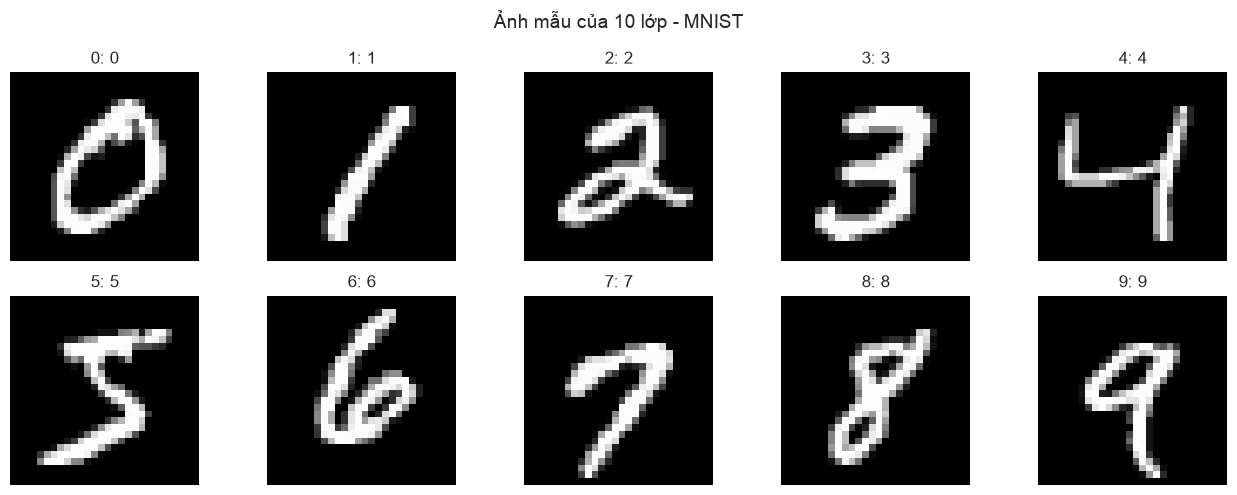
\includegraphics[width=\textwidth]{mnist_sample_images.png}
    \caption{Ảnh mẫu của 10 lớp chữ số trong MNIST}
    \label{fig:mnist_samples}
\end{figure}

Phân phối lớp không hoàn toàn đồng đều nhưng không mất cân bằng nghiêm trọng.
Lớp 1 có 6,742 mẫu train, trong khi lớp 5 có 5,421 mẫu.
Macro-F1 vẫn được dùng để mỗi chữ số có đóng góp ngang nhau vào kết luận.

\begin{figure}[H]
    \centering
    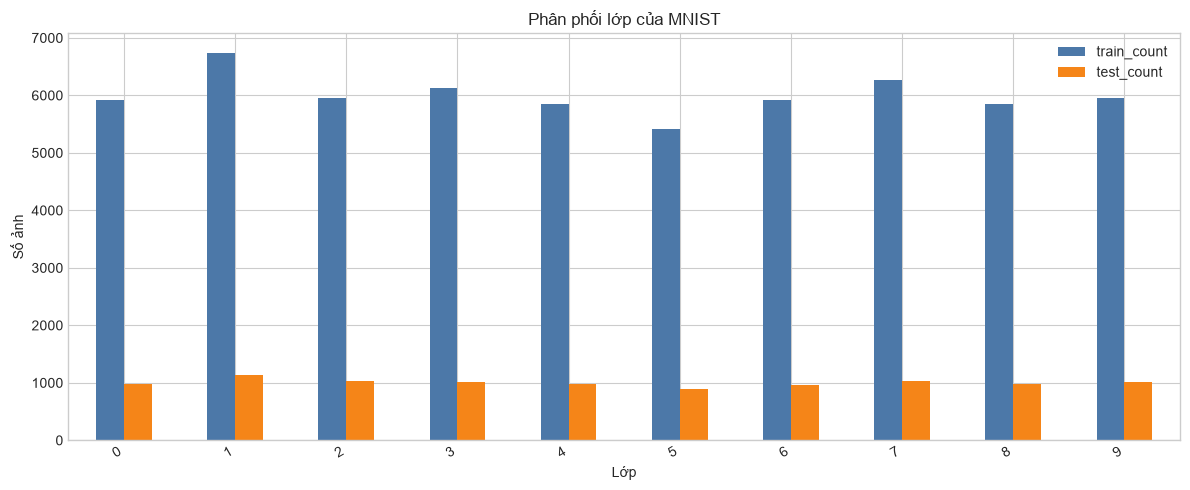
\includegraphics[width=0.95\textwidth]{mnist_class_distribution.png}
    \caption{Phân phối lớp của MNIST trên tập train gốc và test}
    \label{fig:mnist_distribution}
\end{figure}

\section{Tiền xử lý và cấu hình}
Tập train framework có 54,000 mẫu, validation có 6,000 mẫu.
Subset NumPy gồm 20,000 mẫu train và 3,000 mẫu validation, đều lấy stratified từ phần train.
Mean và standard deviation học từ train lần lượt là 0.13073687 và 0.30819046.

CNN NumPy có cấu trúc
$28\times28\times1\to\text{Conv}(8)\to\text{Pool}
\to\text{Conv}(16)\to\text{Pool}\to\text{Dense}(64)\to10$,
tổng cộng 52,138 tham số.

Mô hình Keras và PyTorch tương đương về cấu trúc: hai convolution $3\times3$ trong mỗi block, Batch Normalization, ReLU, max pooling, Dropout, sau đó Dense 128 và output 10 lớp.
Keras báo cáo 468,394 tham số tổng; PyTorch báo cáo 468,010 tham số trainable.

\section{Diễn biến huấn luyện}
\begin{figure}[H]
    \centering
    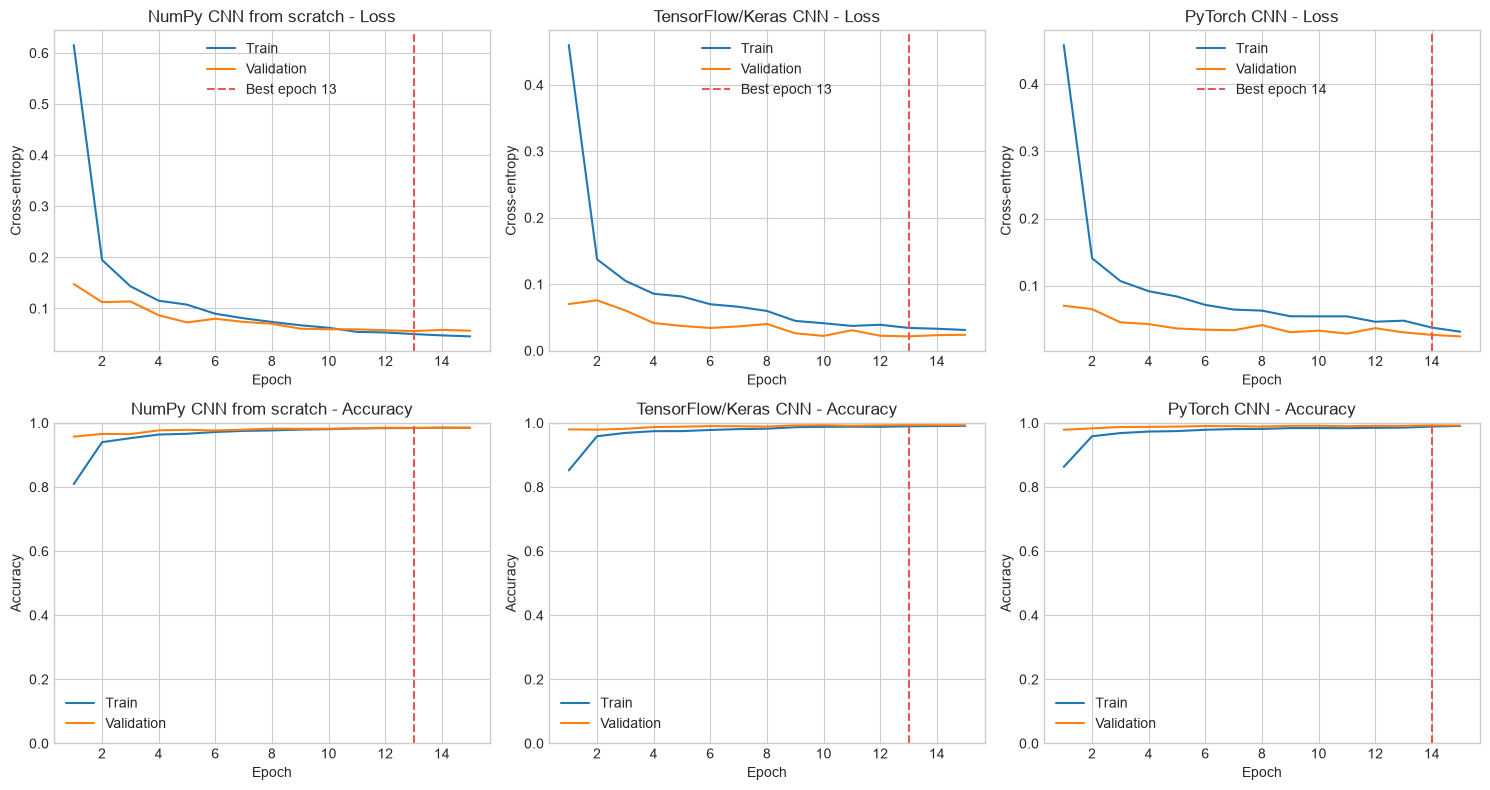
\includegraphics[width=\textwidth]{mnist_learning_curves.png}
    \caption{Learning curves của ba cách cài đặt CNN trên MNIST}
    \label{fig:mnist_learning_curves}
\end{figure}

CNN NumPy giảm validation loss từ 0.1477 ở epoch 1 xuống mức tốt nhất 0.0558 ở epoch 13.
Sau epoch này, validation loss dao động nhẹ dù train loss tiếp tục giảm; khôi phục checkpoint epoch 13 giúp tránh giữ trạng thái cuối kém hơn.

Keras đạt validation accuracy tốt nhất 0.9937 ở epoch 13.
PyTorch đạt validation accuracy tốt nhất 0.9928 ở epoch 14.
Các đường train/validation gần nhau và accuracy đều hội tụ trên 0.99, cho thấy augmentation và regularization kiểm soát overfitting tốt trên MNIST.

\section{Kết quả benchmark}
\begin{table}[H]
\centering
\caption{Benchmark ba cách cài đặt CNN trên MNIST}
\label{tab:mnist_benchmark}
\resizebox{\textwidth}{!}{%
\begin{tabular}{lccccccccc}
\toprule
\textbf{Mô hình} & \textbf{Accuracy} & \textbf{Macro-P} & \textbf{Macro-R} & \textbf{Macro-F1} & \textbf{Train} & \textbf{Epoch tốt} & \textbf{Tham số} & \textbf{Train(s)} & \textbf{Pred(s)} \\
\midrule
PyTorch CNN & \best{0.9958} & \best{0.9959} & \best{0.9958} & \best{0.9958} & 54,000 & 14 & 468,010 & 90.38 & \best{0.307} \\
TensorFlow/Keras CNN & 0.9955 & 0.9955 & 0.9955 & 0.9955 & 54,000 & 13 & 468,394 & 399.87 & 1.183 \\
NumPy CNN from scratch & 0.9848 & 0.9847 & 0.9847 & 0.9847 & 20,000 & 13 & \best{52,138} & \best{82.86} & 1.094 \\
\bottomrule
\end{tabular}%
}
\end{table}

PyTorch đạt Macro-F1 cao nhất 0.9958, nhỉnh hơn Keras 0.0003.
Khoảng cách này rất nhỏ về chất lượng dự báo.
Trong lần chạy đã lưu, PyTorch đồng thời có thời gian dự đoán thấp nhất và thời gian train chỉ 90.38 giây trên MPS.

CNN NumPy đạt accuracy 0.9848 dù chỉ dùng 20,000 mẫu train và 52,138 tham số.
Kết quả này xác nhận forward/backward thủ công hoạt động đúng.
Khoảng cách khoảng 1.1 điểm phần trăm so với framework chủ yếu phản ánh dữ liệu train ít hơn, kiến trúc nhỏ hơn và thiếu các primitive tối ưu mức thấp.

\begin{figure}[H]
    \centering
    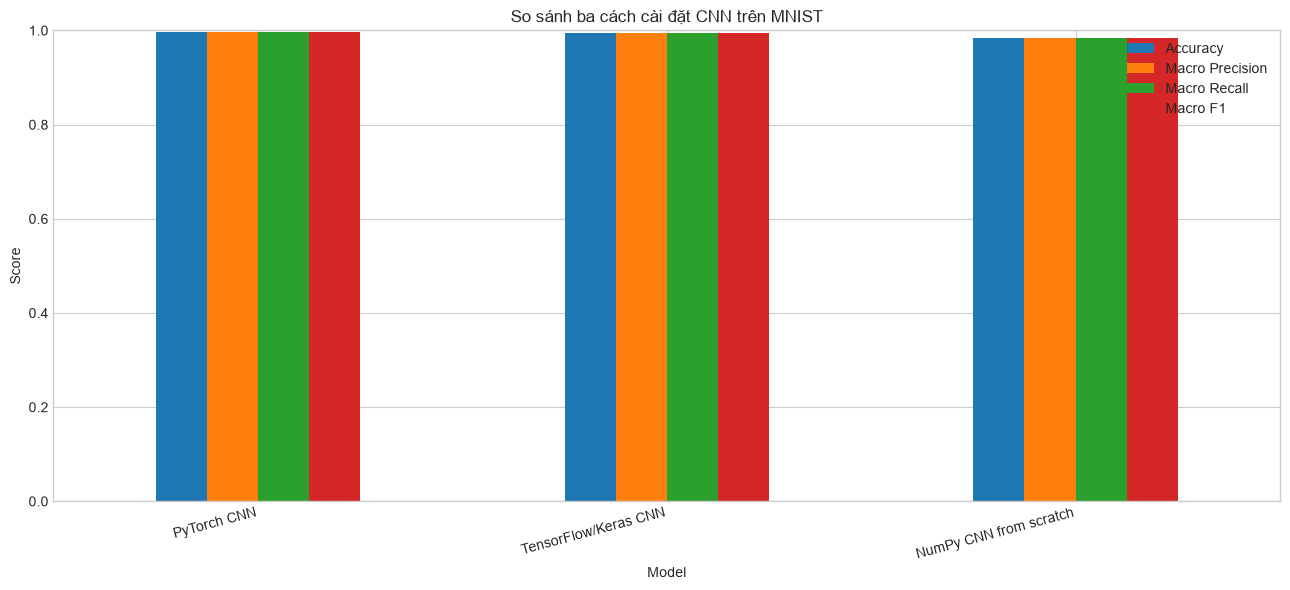
\includegraphics[width=\textwidth]{mnist_metric_comparison.png}
    \caption{So sánh Accuracy, Macro-Precision, Macro-Recall và Macro-F1 trên MNIST}
    \label{fig:mnist_metric_comparison}
\end{figure}

\section{Ma trận nhầm lẫn và phân tích lỗi}
\begin{figure}[H]
    \centering
    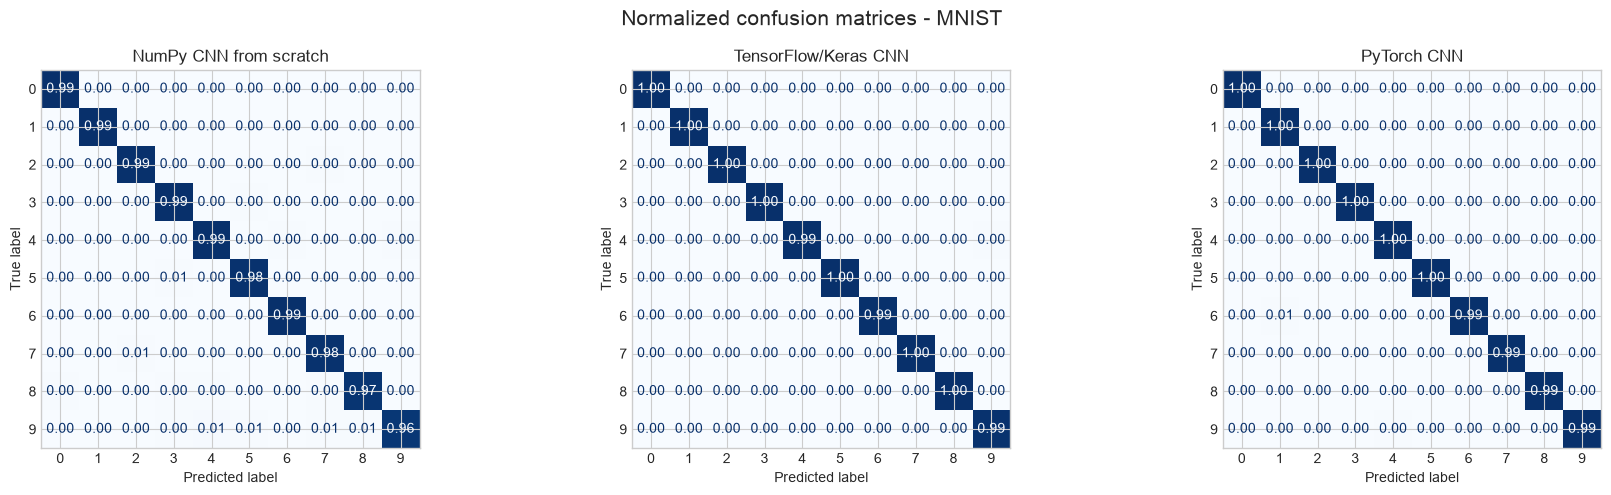
\includegraphics[width=\textwidth]{mnist_normalized_confusion_matrices.png}
    \caption{Ma trận nhầm lẫn chuẩn hóa của ba mô hình trên MNIST}
    \label{fig:mnist_confusion}
\end{figure}

Ma trận của hai framework gần như tập trung hoàn toàn trên đường chéo.
CNN NumPy còn yếu hơn ở chữ số 8 và 9, với recall hiển thị xấp xỉ 0.97 và 0.96.
Điều này phù hợp với việc những chữ số có nét vòng hoặc nét kéo dài dễ bị nhầm khi kiểu viết không điển hình.

\begin{table}[H]
\centering
\caption{Accuracy theo lớp của mô hình tốt nhất trên MNIST (PyTorch CNN)}
\label{tab:mnist_per_class}
\begin{tabular}{crr@{\qquad}crr}
\toprule
\textbf{Lớp} & \textbf{Số mẫu} & \textbf{Accuracy} & \textbf{Lớp} & \textbf{Số mẫu} & \textbf{Accuracy} \\
\midrule
0 & 980 & 0.9990 & 5 & 892 & 0.9955 \\
1 & 1,135 & 0.9974 & 6 & 958 & 0.9927 \\
2 & 1,032 & 0.9971 & 7 & 1,028 & 0.9942 \\
3 & 1,010 & 0.9960 & 8 & 974 & 0.9949 \\
4 & 982 & 0.9990 & 9 & 1,009 & 0.9921 \\
\bottomrule
\end{tabular}
\end{table}

Lớp 0 và 4 đạt accuracy 0.9990; lớp 9 thấp nhất với 0.9921 nhưng vẫn ở mức rất cao.
Hình \ref{fig:mnist_errors} chọn các lỗi có confidence lớn nhất.
Nhiều ảnh có nét viết mơ hồ: chữ số 5 giống 6 hoặc 3, chữ số 7 giống 1, và chữ số 9 bị viết gần giống 4.
Confidence cao không bảo đảm dự đoán đúng khi hình dạng nằm ngoài kiểu phổ biến của tập train.

\begin{figure}[H]
    \centering
    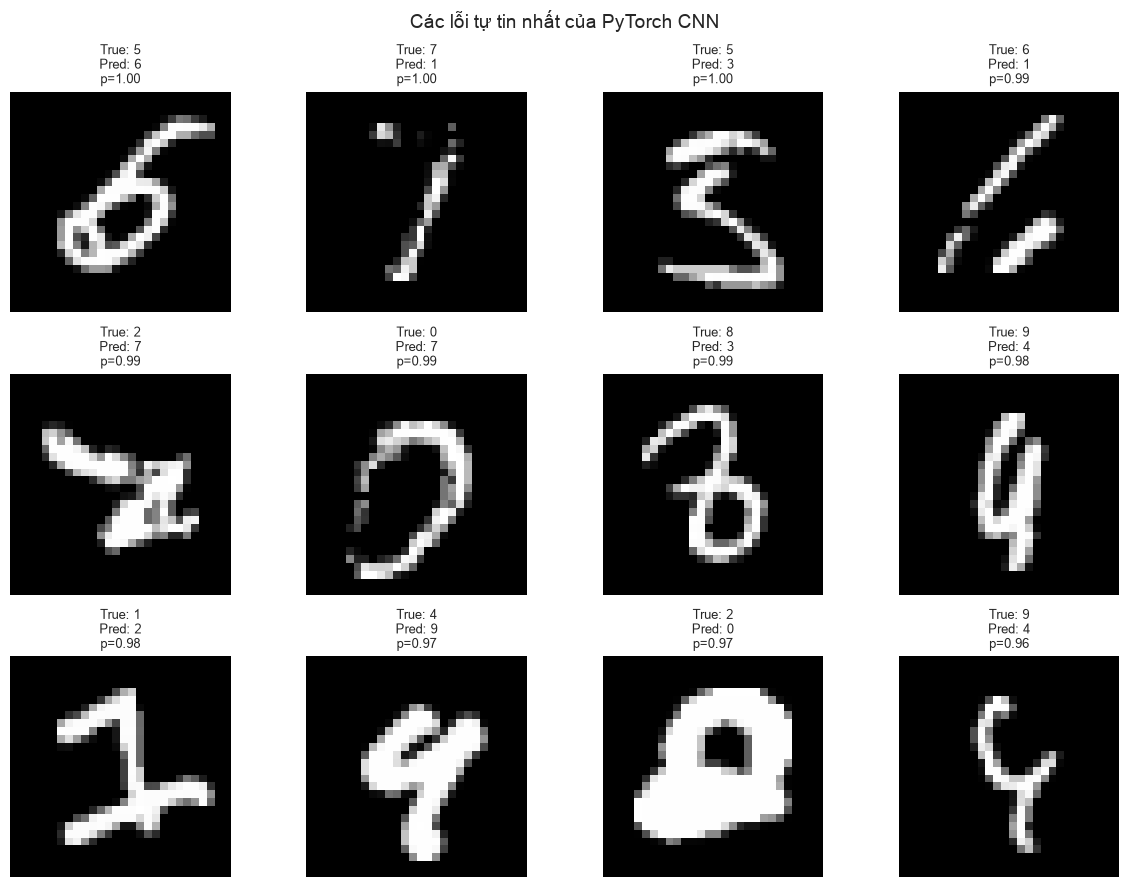
\includegraphics[width=0.88\textwidth]{mnist_prediction_error_analysis.png}
    \caption{Các dự đoán sai có confidence cao nhất của PyTorch CNN trên MNIST}
    \label{fig:mnist_errors}
\end{figure}

% =========================================================================
% CHUONG 4
% =========================================================================
\chapter{Thực Nghiệm Trên CIFAR-10}

\section{Khảo sát dữ liệu}
CIFAR-10 có 50,000 ảnh train và 10,000 ảnh test, chia đều cho mười lớp:
\textit{airplane, automobile, bird, cat, deer, dog, frog, horse, ship, truck}.
Mỗi ảnh chỉ có $32\times32$ pixel nhưng chứa nền tự nhiên, vật thể ở nhiều tỉ lệ và biến đổi ánh sáng.

\begin{figure}[H]
    \centering
    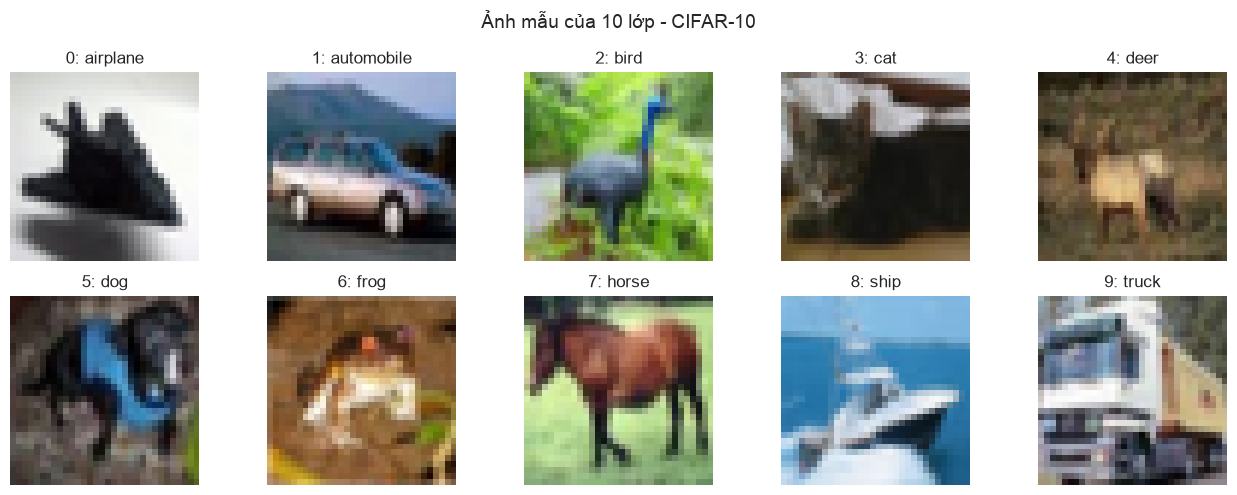
\includegraphics[width=\textwidth]{cifar10_sample_images.png}
    \caption{Ảnh mẫu của 10 lớp trong CIFAR-10}
    \label{fig:cifar_samples}
\end{figure}

\begin{figure}[H]
    \centering
    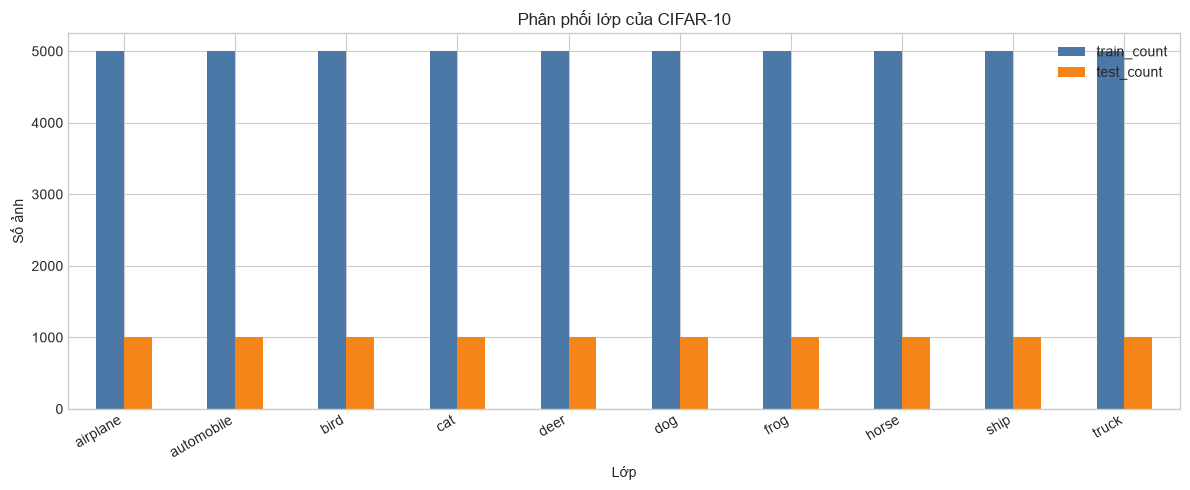
\includegraphics[width=0.95\textwidth]{cifar10_class_distribution.png}
    \caption{Phân phối cân bằng tuyệt đối của CIFAR-10}
    \label{fig:cifar_distribution}
\end{figure}

Mỗi lớp có đúng 5,000 ảnh train gốc và 1,000 ảnh test.
Do dữ liệu cân bằng, Accuracy và Macro-Recall bằng nhau trong bảng kết quả.
Macro-F1 vẫn cần thiết vì precision có thể khác nhau giữa các lớp dễ và khó.

\section{Tiền xử lý và cấu hình}
Tập framework train gồm 45,000 mẫu, validation 5,000 mẫu.
Subset NumPy gồm 15,000 mẫu train và 3,000 mẫu validation, mỗi lớp có đúng 1,500 mẫu NumPy train.
Mean và standard deviation ba channel học từ train là:
\begin{align}
    \boldsymbol{\mu}_{train}
    &= (0.49113446,\ 0.48211210,\ 0.44644734),\\
    \boldsymbol{\sigma}_{train}
    &= (0.24686947,\ 0.24343061,\ 0.26160370).
\end{align}

CNN NumPy dùng 12 và 24 filter, hidden layer 128, tổng 200,978 tham số.
Mô hình này vẫn là CNN hai block nhằm giữ toàn bộ backward khả thi bằng NumPy.
Keras và PyTorch dùng ResNet-20, ba stage $16\to32\to64$, ba residual block mỗi stage và Global Average Pooling.
Số tham số báo cáo tương ứng là 274,042 và 272,474.

\section{Diễn biến huấn luyện}
\begin{figure}[H]
    \centering
    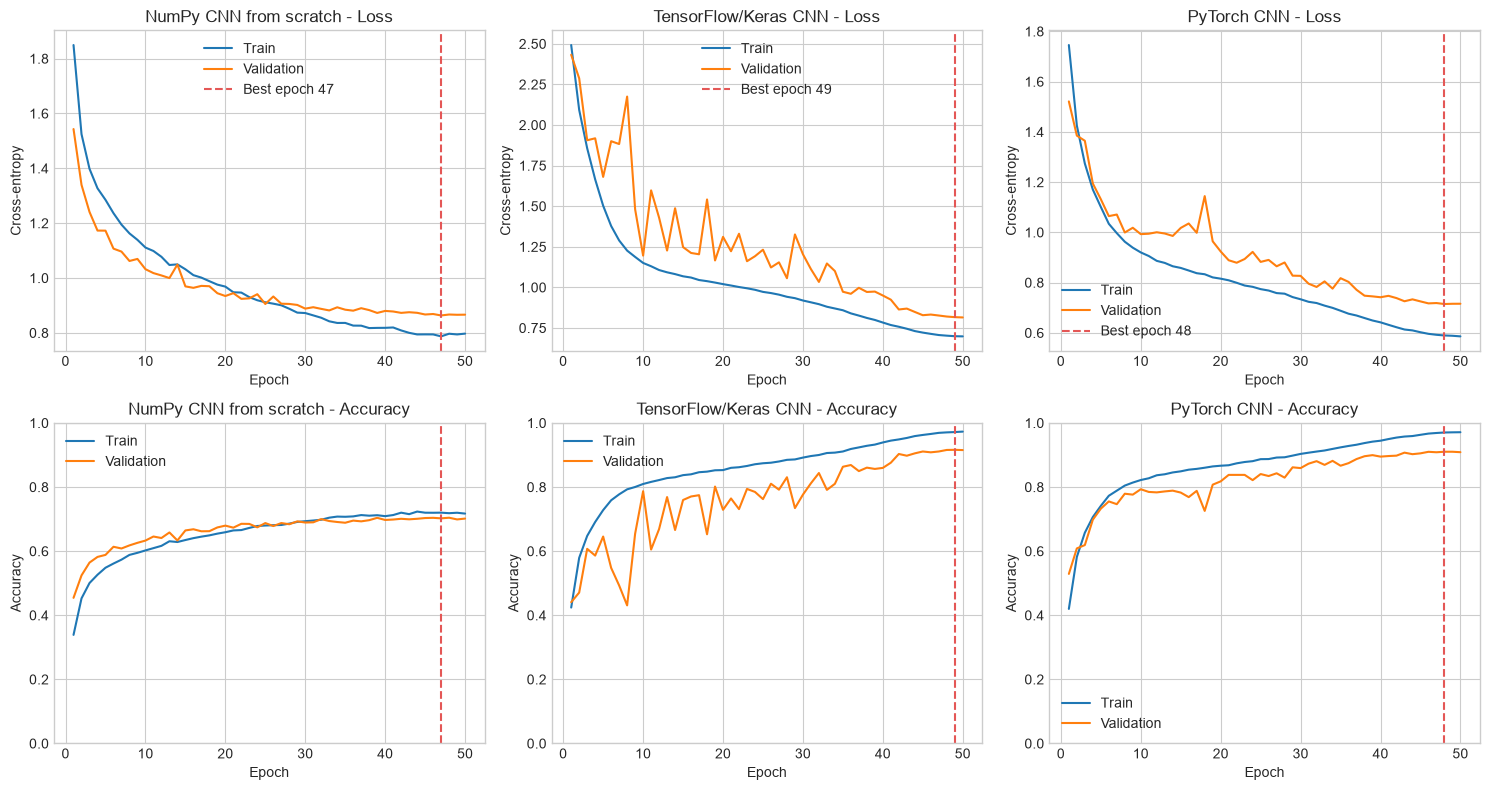
\includegraphics[width=\textwidth]{cifar10_learning_curves.png}
    \caption{Learning curves của ba cách cài đặt CNN trên CIFAR-10}
    \label{fig:cifar_learning_curves}
\end{figure}

CNN NumPy hội tụ chậm và dừng quanh accuracy train/validation 0.72/0.70.
Validation loss tốt nhất là 0.8634 tại epoch 47.
Hai đường train và validation gần nhau cho thấy hạn chế chính là underfitting: kiến trúc nông và subset 15,000 ảnh chưa đủ để học các biến thể phức tạp.

Keras và PyTorch cải thiện rõ sau giai đoạn đầu nhờ residual blocks và lịch learning rate dài.
Keras đạt validation accuracy tốt nhất 0.9162 ở epoch 49; PyTorch đạt 0.9102 ở epoch 48.
Đường validation có dao động trong nửa đầu huấn luyện, phản ánh ảnh hưởng của augmentation mạnh, SGD và learning rate lớn.
Khi cosine decay hạ learning rate về cuối, metric ổn định và đạt vùng tốt nhất.

\section{Kết quả benchmark}
\begin{table}[H]
\centering
\caption{Benchmark ba cách cài đặt CNN trên CIFAR-10}
\label{tab:cifar_benchmark}
\resizebox{\textwidth}{!}{%
\begin{tabular}{lccccccccc}
\toprule
\textbf{Mô hình} & \textbf{Accuracy} & \textbf{Macro-P} & \textbf{Macro-R} & \textbf{Macro-F1} & \textbf{Train} & \textbf{Epoch tốt} & \textbf{Tham số} & \textbf{Train(s)} & \textbf{Pred(s)} \\
\midrule
PyTorch CNN & \best{0.9095} & \best{0.9092} & \best{0.9095} & \best{0.9092} & 45,000 & 48 & 272,474 & 822.82 & \best{1.248} \\
TensorFlow/Keras CNN & 0.9078 & 0.9077 & 0.9078 & 0.9075 & 45,000 & 49 & 274,042 & 2,636.45 & 4.125 \\
NumPy CNN from scratch & 0.7012 & 0.6987 & 0.7012 & 0.6994 & 15,000 & 47 & \best{200,978} & \best{501.36} & 3.875 \\
\bottomrule
\end{tabular}%
}
\end{table}

PyTorch có Macro-F1 cao nhất 0.9092, hơn Keras 0.0017.
Hai phiên bản ResNet-20 vì vậy gần tương đương về chất lượng, nhưng khác đáng kể về thời gian trong lần chạy này.
PyTorch train 822.82 giây và dự đoán 1.248 giây; Keras train 2,636.45 giây và dự đoán 4.125 giây.
Kết quả thời gian phụ thuộc backend, MPS, compilation và trạng thái máy nên không nên khái quát thành ưu thế tuyệt đối của framework.

CNN NumPy đạt Macro-F1 0.6994.
So với ResNet-20, khoảng cách lớn cho thấy CIFAR-10 hưởng lợi mạnh từ độ sâu, residual connection, Batch Normalization, Global Average Pooling, full train set và chính sách tối ưu chuyên biệt.

\begin{figure}[H]
    \centering
    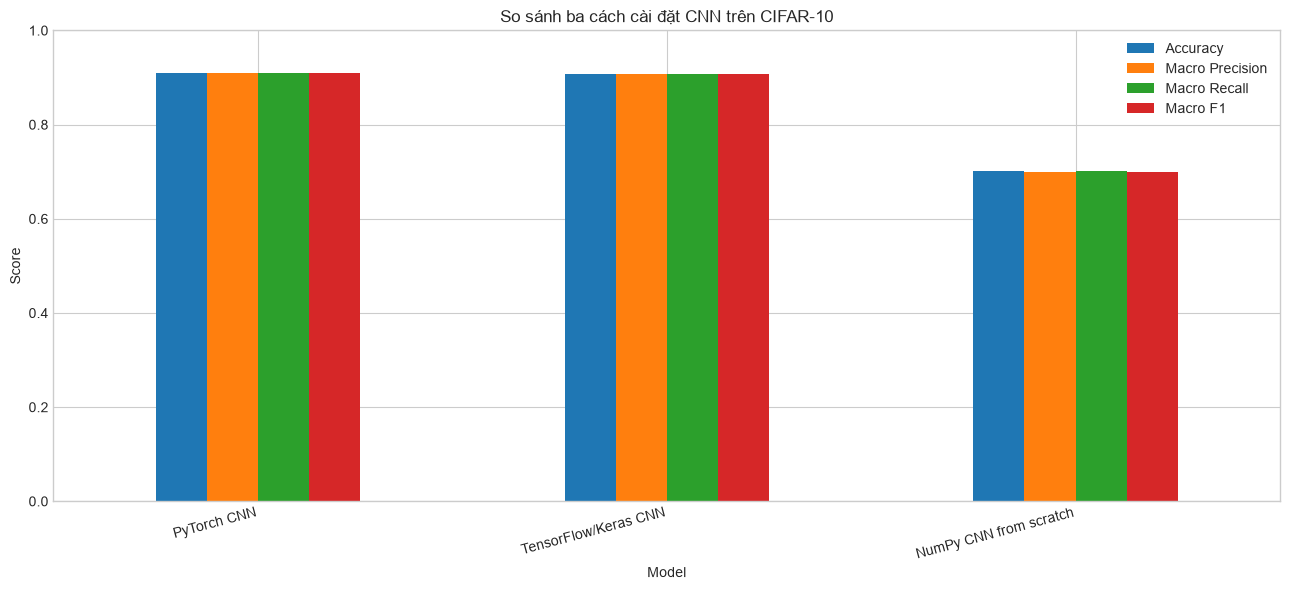
\includegraphics[width=\textwidth]{cifar10_metric_comparison.png}
    \caption{So sánh Accuracy, Macro-Precision, Macro-Recall và Macro-F1 trên CIFAR-10}
    \label{fig:cifar_metric_comparison}
\end{figure}

\section{Ma trận nhầm lẫn và độ khó theo lớp}
\begin{figure}[H]
    \centering
    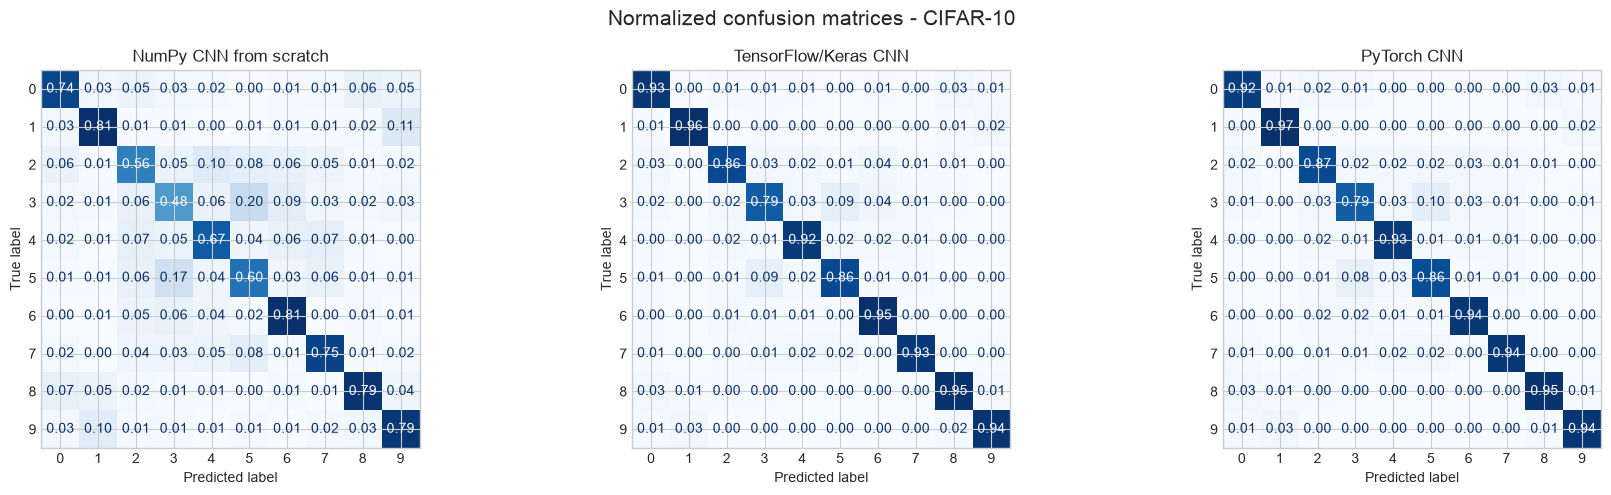
\includegraphics[width=\textwidth]{cifar10_normalized_confusion_matrices.png}
    \caption{Ma trận nhầm lẫn chuẩn hóa của ba mô hình trên CIFAR-10}
    \label{fig:cifar_confusion}
\end{figure}

CNN NumPy nhầm nhiều giữa các lớp động vật.
Trong ma trận đã làm tròn, recall lớp \textit{cat} chỉ khoảng 0.48 và 20\% ảnh mèo bị dự đoán thành chó.
Lớp \textit{bird} cũng dễ nhầm sang \textit{deer}, \textit{dog} hoặc \textit{frog}.
Các lớp phương tiện có đường nét và bối cảnh đặc trưng hơn nên nhìn chung dễ phân loại hơn.

ResNet-20 giảm mạnh các ô ngoài đường chéo nhưng cặp \textit{cat}--\textit{dog} vẫn là nguồn lỗi lớn nhất.
Đây là cặp có texture, tư thế và bối cảnh tương tự ở độ phân giải thấp.

\begin{table}[H]
\centering
\caption{Accuracy theo lớp của mô hình tốt nhất trên CIFAR-10 (PyTorch CNN)}
\label{tab:cifar_per_class}
\begin{tabular}{lrr@{\qquad}lrr}
\toprule
\textbf{Lớp} & \textbf{Số mẫu} & \textbf{Accuracy} & \textbf{Lớp} & \textbf{Số mẫu} & \textbf{Accuracy} \\
\midrule
airplane & 1,000 & 0.9150 & dog & 1,000 & 0.8560 \\
automobile & 1,000 & \best{0.9660} & frog & 1,000 & 0.9390 \\
bird & 1,000 & 0.8660 & horse & 1,000 & 0.9360 \\
cat & 1,000 & 0.7940 & ship & 1,000 & 0.9510 \\
deer & 1,000 & 0.9290 & truck & 1,000 & 0.9430 \\
\bottomrule
\end{tabular}
\end{table}

Lớp \textit{automobile} tốt nhất với accuracy 0.9660; \textit{cat} thấp nhất với 0.7940.
Khoảng cách 17.2 điểm phần trăm giữa hai lớp cho thấy score tổng hợp 0.9095 không phản ánh đầy đủ sự khác nhau theo ngữ nghĩa.

\section{Phân tích lỗi confidence cao}
\begin{figure}[H]
    \centering
    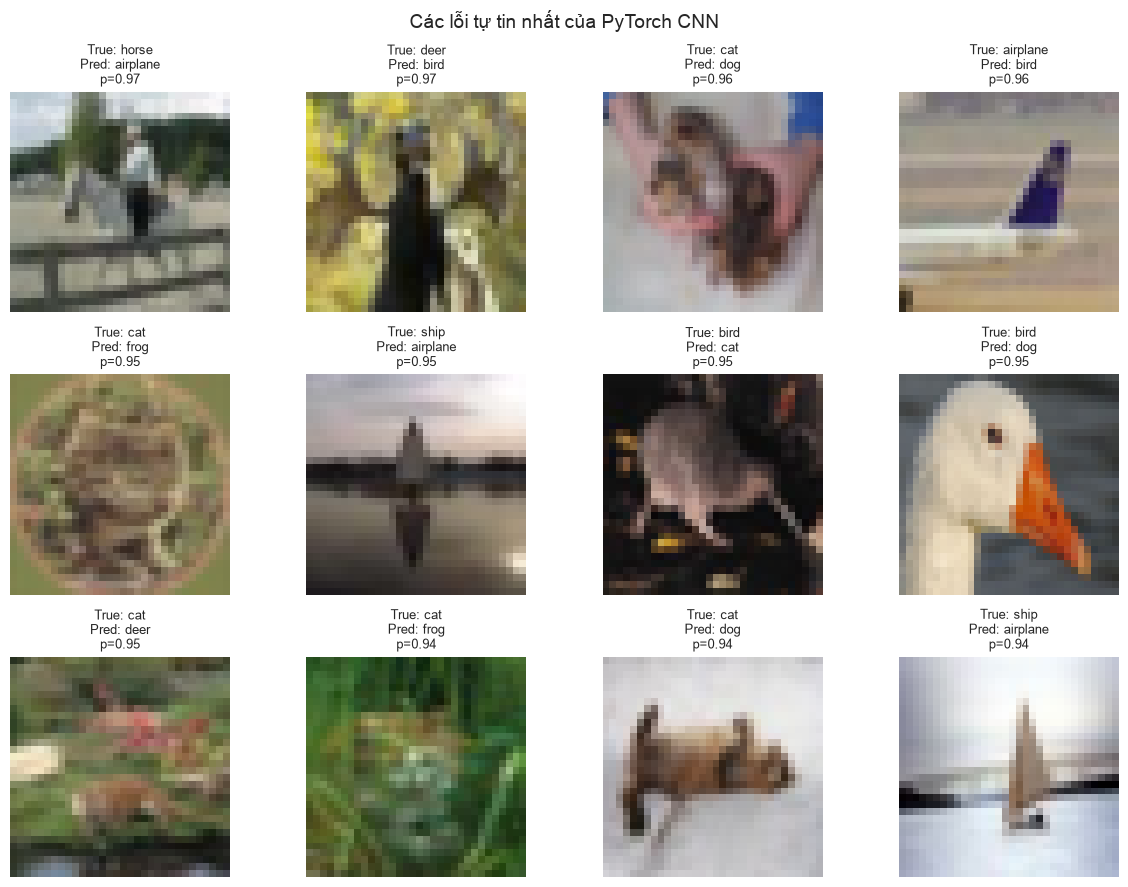
\includegraphics[width=0.88\textwidth]{cifar10_prediction_error_analysis.png}
    \caption{Các dự đoán sai có confidence cao nhất của PyTorch CNN trên CIFAR-10}
    \label{fig:cifar_errors}
\end{figure}

Nhiều lỗi confidence cao có tính mơ hồ thực sự ở độ phân giải $32\times32$:
ngựa bị che khuất giống máy bay, hươu trong nền rừng giống chim, mèo/chó/chim bị nhầm lẫn do texture, hoặc thuyền và máy bay cùng xuất hiện trên nền trời/nước.
Những ví dụ này chỉ ra rằng xác suất softmax cao không đồng nghĩa mô hình đã được hiệu chỉnh xác suất tốt.
Trong một hệ thống thực tế, có thể bổ sung calibration, dự đoán top-$k$ hoặc cơ chế từ chối khi độ tin cậy không đáng tin cậy.

% =========================================================================
% CHUONG 5
% =========================================================================
\chapter{Tổng Hợp Đối Chuẩn Và Kết Luận}

\section{Tổng hợp kết quả chính}
\begin{table}[H]
\centering
\caption{Tổng hợp mô hình tốt nhất và CNN NumPy trên hai dataset}
\label{tab:master_summary}
\resizebox{\textwidth}{!}{%
\begin{tabular}{lllllll}
\toprule
\textbf{Dataset} & \textbf{Mô hình} & \textbf{Accuracy} & \textbf{Macro-F1} & \textbf{Tham số} & \textbf{Train(s)} & \textbf{Dữ liệu train} \\
\midrule
MNIST & PyTorch CNN & 0.9958 & 0.9958 & 468,010 & 90.38 & 54,000 \\
MNIST & NumPy CNN & 0.9848 & 0.9847 & 52,138 & 82.86 & 20,000 \\
CIFAR-10 & PyTorch ResNet-20 & 0.9095 & 0.9092 & 272,474 & 822.82 & 45,000 \\
CIFAR-10 & NumPy CNN & 0.7012 & 0.6994 & 200,978 & 501.36 & 15,000 \\
\bottomrule
\end{tabular}%
}
\end{table}

Trên MNIST, một CNN nông đã đủ mạnh: NumPy chỉ kém framework khoảng 1.1 điểm phần trăm accuracy.
Trên CIFAR-10, cùng cách cài đặt nông bị giới hạn ở khoảng 70\%, trong khi ResNet-20 vượt 90\%.
So sánh này minh họa rằng độ phức tạp kiến trúc cần phù hợp độ phức tạp dữ liệu.

\section{So sánh ba cách cài đặt}
\begin{table}[H]
\centering
\caption{Ưu và nhược điểm của ba cách cài đặt CNN}
\label{tab:implementation_tradeoff}
\resizebox{\textwidth}{!}{%
\begin{tabular}{llll}
\toprule
\textbf{Cách cài đặt} & \textbf{Ưu điểm} & \textbf{Hạn chế} & \textbf{Vai trò trong Assignment 04} \\
\midrule
NumPy from scratch & Minh bạch forward/backward, ít phụ thuộc & Chậm, khó mở rộng, dễ sai gradient & Hiểu thuật toán ở mức tensor \\
TensorFlow/Keras & API gọn, callback và pipeline dữ liệu tốt & Training loop ít tường minh hơn & Xây dựng baseline framework nhanh \\
PyTorch & Module và loop linh hoạt, debug thuận tiện & Cần tự quản lý nhiều trạng thái & Benchmark hiệu quả và kiểm soát rõ \\
\bottomrule
\end{tabular}%
}
\end{table}

CNN NumPy không nhằm thay thế framework trong triển khai quy mô lớn.
Giá trị chính của nó là phơi bày gradient, cache, phép im2col/sliding window, mask pooling và cập nhật Adam.
Keras và PyTorch phù hợp hơn khi cần residual blocks, tăng tốc phần cứng, mixed precision hoặc mở rộng sang dữ liệu lớn.

\section{Công bằng và giới hạn của benchmark}
Benchmark giữ cùng validation/test set và metric, nhưng không phải mọi điều kiện đều giống hệt:
\begin{enumerate}
    \item NumPy dùng ít mẫu train hơn framework để giới hạn thời gian chạy.
    \item Kiến trúc NumPy nông hơn, còn CIFAR-10 framework dùng ResNet-20.
    \item Số tham số Keras gồm cả trạng thái không trainable của Batch Normalization, trong khi PyTorch đếm tham số trainable.
    \item Thời gian chịu ảnh hưởng của MPS, backend, graph compilation, warm-up và tải hệ thống tại thời điểm chạy.
    \item Chỉ một random seed được báo cáo; chưa có trung bình và độ lệch chuẩn qua nhiều lần chạy.
\end{enumerate}

Vì vậy bảng kết quả trả lời câu hỏi ``pipeline nào hiệu quả trong cấu hình notebook này'' hơn là chứng minh framework nào luôn nhanh hoặc luôn chính xác hơn.

\section{Kiểm toán khả năng tái lập}
\begin{table}[H]
\centering
\caption{Checklist tái lập Assignment 04}
\label{tab:reproducibility}
\resizebox{\textwidth}{!}{%
\begin{tabular}{lll}
\toprule
\textbf{Hạng mục} & \textbf{Cách thực hiện} & \textbf{Ý nghĩa} \\
\midrule
Random seed & \texttt{RANDOM\_STATE = 42} cho NumPy/Keras/Torch & Giảm dao động split và khởi tạo \\
Tách dữ liệu & Stratified train/validation, test độc lập & Không chọn mô hình trên test \\
Chuẩn hóa & Mean/std chỉ học từ framework train & Chống data leakage \\
Checkpoint & NumPy theo val loss, framework theo val accuracy & Khôi phục trạng thái tốt nhất \\
Augmentation & Chỉ áp dụng cho mini-batch train & Giữ validation/test nguyên bản \\
Metric & Accuracy và macro P/R/F1 trên cùng test set & So sánh đa chiều \\
Hình ảnh & Lưu PNG từ output notebook & Truy vết được bảng và đồ thị \\
\bottomrule
\end{tabular}%
}
\end{table}

Trong output đã lưu, môi trường báo cáo NumPy 2.5.2, TensorFlow 2.21.0 và PyTorch 2.14.0.
Để đối chiếu đúng thời gian, cần chạy lại trên cùng kernel và thiết bị; để đối chiếu score, quan trọng nhất là giữ seed, split, preprocessing và cấu hình epoch.

\subsection{Thứ tự chạy lại notebook}
\begin{enumerate}
    \item Mở notebook từ thư mục \modelpath{src/Assignment 04/<dataset>/notebook}.
    \item Kiểm tra dữ liệu cục bộ trong thư mục \modelpath{../data} và các phiên bản thư viện.
    \item Chạy toàn bộ cell theo thứ tự: cấu hình, load dữ liệu, split/normalize, NumPy, Keras, PyTorch, benchmark và error analysis.
    \item Kiểm tra các file PNG trong \modelpath{report/figures}, sau đó đồng bộ vào thư mục ảnh của báo cáo.
    \item Biên dịch file này bằng XeLaTeX ít nhất hai lần để cập nhật mục lục và tham chiếu chéo.
\end{enumerate}

\section{Kết luận}
Báo cáo đã xây dựng và đối chuẩn ba cách cài đặt CNN trên MNIST và CIFAR-10.
Các kết quả chính gồm:
\begin{enumerate}
    \item CNN thuần NumPy hiện thực đầy đủ forward, backward, Adam, weight decay, gradient clipping, cosine learning rate và augmentation.
    \item Trên MNIST, PyTorch đạt Accuracy/Macro-F1 0.9958; Keras đạt 0.9955; NumPy đạt Accuracy 0.9848 và Macro-F1 0.9847.
    \item Trên CIFAR-10, PyTorch ResNet-20 đạt Accuracy 0.9095 và Macro-F1 0.9092; Keras gần tương đương; CNN NumPy nông đạt Macro-F1 0.6994.
    \item Residual connection, Batch Normalization, augmentation, label smoothing và lịch learning rate dài tạo khác biệt rõ trên dữ liệu ảnh tự nhiên.
    \item Error analysis cho thấy các lớp có hình dạng/texture gần nhau vẫn dễ bị nhầm, đặc biệt \textit{cat} và \textit{dog} trên CIFAR-10.
\end{enumerate}

Hướng mở rộng gồm chạy nhiều seed để báo cáo độ ổn định, kiểm tra calibration, thử mixup/cutout, dùng transfer learning và đo thêm throughput, bộ nhớ cùng kích thước checkpoint.
Với CNN NumPy, có thể vector hóa convolution sâu hơn hoặc dùng Numba/CuPy để tách ảnh hưởng của thuật toán khỏi overhead vòng lặp Python.

\end{document}
